\documentclass[10pt]{exam}

\usepackage{amssymb, amsmath, amsthm, mathrsfs, multicol, graphicx}
\usepackage{tikz}

 \def\d{\displaystyle}
\def\?{\reflectbox{?}}
\def\b#1{\mathbf{#1}}
\def\f#1{\mathfrak #1}
\def\c#1{\mathcal #1}
\def\s#1{\mathscr #1}
\def\r#1{\mathrm{#1}}
\def\N{\mathbb N}
\def\Z{\mathbb Z}
\def\Q{\mathbb Q}
\def\R{\mathbb R}
\def\C{\mathbb C}
\def\F{\mathbb F}
\def\A{\mathbb A}
\def\X{\mathbb X}
\def\E{\mathbb E}
\def\O{\mathbb O}
\def\U{\mathcal U}
\def\pow{\mathcal P}
\def\inv{^{-1}}
\def\nrml{\triangleleft}
\def\st{:}
\def\~{\widetilde}
\def\rem{\mathcal R}
\def\sigalg{$\sigma$-algebra }
\def\Gal{\mbox{Gal}}
\def\iff{\leftrightarrow}
\def\Iff{\Leftrightarrow}
\def\land{\wedge}
\def\And{\bigwedge}
\def\AAnd{\d\bigwedge\mkern-18mu\bigwedge}
\def\Vee{\bigvee}
\def\VVee{\d\Vee\mkern-18mu\Vee}
\def\imp{\rightarrow}
\def\Imp{\Rightarrow}
\def\Fi{\Leftarrow}

%\def\={\equiv}
\def\var{\mbox{var}}
\def\mod{\mbox{Mod}}
\def\Th{\mbox{Th}}
\def\sat{\mbox{Sat}}
\def\con{\mbox{Con}}
\def\bmodels{=\joinrel\mathrel|}
\def\iffmodels{\bmodels\models}
\def\dbland{\bigwedge \!\!\bigwedge}
\def\dom{\mbox{dom}}
\def\rng{\mbox{range}}
\DeclareMathOperator{\wgt}{wgt}


\def\bar{\overline}


\newcommand{\vtx}[2]{node[fill,circle,inner sep=0pt, minimum size=4pt,label=#1:#2]{}}
\newcommand{\va}[1]{\vtx{above}{#1}}
\newcommand{\vb}[1]{\vtx{below}{#1}}
\newcommand{\vr}[1]{\vtx{right}{#1}}
\newcommand{\vl}[1]{\vtx{left}{#1}}
\renewcommand{\v}{\vtx{above}{}}

\def\circleA{(-.5,0) circle (1)}
\def\circleAlabel{(-1.5,.6) node[above]{$A$}}
\def\circleB{(.5,0) circle (1)}
\def\circleBlabel{(1.5,.6) node[above]{$B$}}
\def\circleC{(0,-1) circle (1)}
\def\circleClabel{(.5,-2) node[right]{$C$}}
\def\twosetbox{(-2,-1.4) rectangle (2,1.4)}
\def\threesetbox{(-2.5,-2.4) rectangle (2.5,1.4)}
\newcommand{\twoline}[2]{\begin{pmatrix}#1 \\ #2 \end{pmatrix}}


\def\circleA{(-.5,0) circle (1)}
\def\circleAlabel{(-1.5,.6) node[above]{$A$}}
\def\circleB{(.5,0) circle (1)}
\def\circleBlabel{(1.5,.6) node[above]{$B$}}
\def\circleC{(0,-1) circle (1)}
\def\circleClabel{(.5,-2) node[right]{$C$}}
\def\twosetbox{(-2,-1.5) rectangle (2,1.5)}
\def\threesetbox{(-2,-2.5) rectangle (2,1.5)}


%\pointname{pts}
\pointsinmargin
\marginpointname{pts}
\marginbonuspointname{pts-bns}
\addpoints
\pagestyle{head}
\printanswers

\firstpageheader{Math 228}{\textbf{Homework 5 Solutions}}{Due: Wednesday, September 26}


\begin{document}
% \noindent \textbf{Instructions}: Same rules as usual.  Write up solutions on separate sheets of paper; you may work together to understand the problems, but write up your solutions individually.  You may NOT look for solutions online or in other books.

\begin{questions}
  \question[18] Consider the graph below, call it $G$.

  \begin{center}
    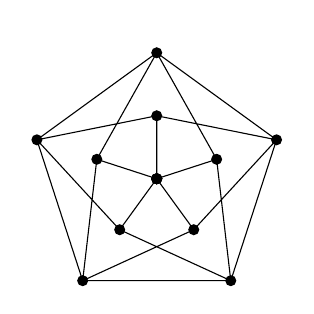
\begin{tikzpicture}[scale=0.8]
      \foreach \x in {0,...,4}{
    \draw (0,0) \v -- (90+\x*72:1) \v -- (162+\x*72:2) \v -- (90+\x*72:2) -- (162+\x*72:1);
    }
    \end{tikzpicture}
  \end{center}
\begin{parts}
  \part Give a careful proof that $G$ is not planar.  Make sure you explain where every equation or inequality you use comes from.
  \begin{solution}
     $G$ has $v = 11$ vertices, $e = 20$ edges, so by Euler's formula, if the graph were planar, it would have $f = 2 + 20 - 11 = 11$ faces.  Also the new graph does not have any triangles, so its girth is 4.  So every face is bounded by at least 4 edges, but this double counts the edges, so we have $4f \le 2e$. But this says $44 \le 40$, a contradiction.
  \end{solution}
  \part Explain why we cannot use the same sort of proof we did in part (a) to prove that the graph $G'$ below is not planar.  Then explain how you know the graph is not planar anyway.
  \begin{center}
    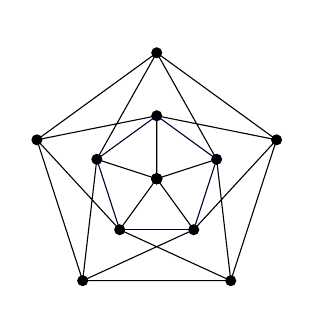
\begin{tikzpicture}[scale=0.8]
      \foreach \x in {0,...,4}{
      \draw (0,0) \v -- (90+\x*72:1) \v -- (162+\x*72:2) \v -- (90+\x*72:2) -- (162+\x*72:1);
      \draw[black!80!blue] (90+\x*72:1) -- (162+\x*72:1);
      }
    \end{tikzpicture}
  \end{center}
  \begin{solution}
    If you try to use Euler's formula and the girth inequality, you do not get a contradiction: $v = 11$, $e = 25$, so $f = 2 + 25 - 11 = 16$, but here the girth is 3, so $3f \le 2e$, which says that $48 \le 50$ (which is true).  However, if you remove some edges to increase the girth, you could use this proof technique.  In particular, remove the five edges of the inner pentagon, you get $G$ above.

    If $G'$ \emph{was} planar, then so would all of its subgraphs.  But $G$ is a subgraph of $G'$, and $G$ is not planar, so neither is $G$.
  \end{solution}
  \part Find the chromatic number of $G$ (the original graph).  Carefully explain how you know you are correct.
  \begin{solution}
    The chromatic number is 4.  It is not too difficult to find a proper 4-coloring.  To prove that you cannot do better, assume there was a proper 3-coloring.  The outside pentagon will then use all three colors.  In fact, it will necessarily use one color (say red) once, and the other two colors (blue and green) twice.  By rotating the graph, you could assume the red vertex is at the top.
    \begin{center}
      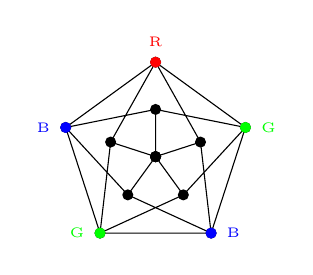
\begin{tikzpicture}[scale=0.6]
        \foreach \x in {0,...,4}{
      \draw (0,0) \v -- (90+\x*72:1) \v -- (162+\x*72:2) \v -- (90+\x*72:2) -- (162+\x*72:1);
      }
      \draw[red] (90:2) \va{\tiny R};
      \draw[blue] (162:2) \vl{\tiny B} (-54:2) \vr{\tiny B};
      \draw[green] (234:2) \vl{\tiny G} (18:2) \vr{\tiny G};
      \end{tikzpicture}
      \hspace{3em}
      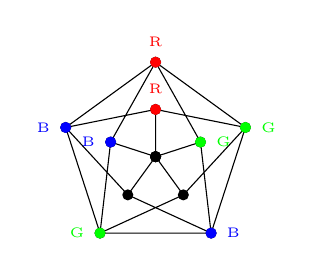
\begin{tikzpicture}[scale=0.6]
        \foreach \x in {0,...,4}{
      \draw (0,0) \v -- (90+\x*72:1) \v -- (162+\x*72:2) \v -- (90+\x*72:2) -- (162+\x*72:1);
      }
      \draw[red] (90:2) \va{\tiny R} (90:1) \va{\tiny R};
      \draw[blue] (162:2) \vl{\tiny B} (162:1) \vl{\tiny B} (-54:2) \vr{\tiny B};
      \draw[green] (234:2) \vl{\tiny G} (18:2) \vr{\tiny G} (18:1) \vr{\tiny G};
      \end{tikzpicture}
    \end{center}

    Now look at the five vertices inside the pentagon.  The top three of these must be three different colors (in fact, the same color as the outer vertex they are closest to).  But that means the center vertex cannot be colored with any of the three colors.

    Note that you cannot use the 4-color theorem, Brooke's theorem, or the clique number here.  (The graph $G$ is called the Grötzsch graph, which is the smallest graph with chromatic number 4 that does not contain any triangles.)
  \end{solution}
\end{parts}


\question[6] Give a careful proof by induction on the number of vertices, that all trees with at least two vertices have chromatic number 2.  You may assume the result that all trees have at least one vertex of degree 1.  Make sure you do the induction step in the correct direction: you must prove that \emph{all} trees with $k+1$ vertices have chromatic number 2, not just those you can get from a particular tree with $k$ vertices.

\begin{solution}
  Let $P(n)$ be the statement, ``Every tree with $n$ vertices has chromatic number 2.''  We will prove $P(n)$ is true for all $n \ge 2$.

  Base case: When $n = 2$, there is only one tree to consider, and anyway, since it only has two vertices, its chromatic number could not be more than 2 (and since the graph is connected, the chromatic number could not be 1).

  Inductive case: Fix $k \ge 2$ at assume $P(k)$ is true.  That is, assume that all trees with $k$ vertices have chromatic number 2.  Now consider an arbitrary tree $T$ with $k+1$ vertices.  Let $v_0$ be a vertex with degree 1, and let $T'$ be the tree you get by removing $v_0$ and its incident edge from $T$.  Then $T'$ has $k$ vertices, so has a proper 2-coloring.

  Color the vertices of $T$ other than $v_0$ using this 2-coloring.  We now need to color $v_0$.  But since $v_0$ only has one neighbor, we can color $v_0$ with the other color, getting a proper 2-coloring of $T$.  Thus $T$ has chromatic number $2$.  This proves that $P(k+1)$ is true.

  Therefore, by the principle of mathematical induction, all trees with at least two vertices have chromatic number 2.
\end{solution}


  \question[6] The two problems below can be solved using graph coloring.  For each problem, represent the situation with a graph, say whether you should be coloring vertices or edges and why, and use the coloring to solve the problem.
  \begin{parts}
    \part Your Quidditch league has 5 teams.  You will play a tournament next week in which every team will play every other team once.  Each team can play at most one match each day, but there is plenty of time in the day for multiple matches.  What is the fewest number of days over which the tournament can take place?

    \begin{solution}
      The graph to represent this question is $K_5$, since each vertex (team) is adjacent to (plays) each other vertex (team).  The edges are thus the games that are played.  We cannot have a team play more than one game per day, so we color the edges observing the rule that two edges incident to the same vertex must be colored differently.  Edges that are colored the same \emph{can} be played on the same day, so we are looking for the smallest number of colors needed to color the edges in this way.  You obviously need at least 4 colors, but 4 colors does not work.  In fact, there is a coloring using 5 colors, so you need 5 days for the tournament.
    \end{solution}
    \part Ten members of Math Club are driving to a math conference in a neighboring state.  However, some of these students have dated in the past, and things are still a little awkward.  Each student lists which other students they refuse to share a car with; these conflicts are recored in the table below.  What is the fewest number of cars the club needs to make the trip?  Do not worry about running out of seats, just avoid the conflicts.

    \begin{tabular}{l|*{10}{c}}
      Student: & A & B & C & D & E & F & G & H & I & J \\ \hline
      Conflicts: &BEJ&ADG&HJ&BF&AI&DJ&B&CI&EHJ&ACFI
    \end{tabular}
    \begin{solution}
      Here we color the vertices.  The chromatic number of this graph is 3, so three cars are needed.
    \end{solution}
  \end{parts}
\end{questions}




\end{document}
